% !Mode\dots ``TeX:UTF-8''

\section{Experiments}
\label{sec:exp}

\subsection{Environment}
We first explain the implementation and computation environment.
\begin{comment}
{\bf Old environment}\ \ \
The main algorithm for isolating real roots based on our improvements has been implemented as a \texttt{C} program, \froot \footnote{The program can be downloaded through \url{https://github.com/djuanbei/logcf}}. Compilation was done using {\tt gcc} version 4.6.3 with optimization flags -O2.
We use {\tt Singular} \cite{singular} to read polynomials from files or standard input and to eliminate multi-factors of polynomials. We use the GMP\footnote{ \url{http://gmplib.org/}}
(version 5.05), arbitrary-length integers libraries, to deal with big integer computation.
Some tests were done before 2014   on a 64-bit Intel(R) Core(TM) i5 CPU 650 @ 3.20GHz with 4GB RAM memory and Ubuntu 12.04 GNU/Linux.
\end{comment}
 We compare \froot\ with \SLV, \AND, \MM's\footnote{11.1 version} \inte\  and  \MAPLE's\footnote{Maple(TM) 2017,Windows(R) (64-bit)} \REALROOT\  on   a 64-bit Intel(R) Core(TM) i7 CPU-4710Q @ 2.50GHz with 8GB RAM memory and Windows 7. In this environment \froot\ was compiled by visual studio 2013.

\subsection{Tricks}
{\bf Variable substitution}
If $p(x)\in \ZZ[x]$ and $p(x)=p_1(x^k)\ (k>1),$ then substitute $y=x^k$ in $p$. Obviously, $\deg(p_1,y)=\frac{\deg(p,x)}{k}$. We first isolate the real roots of $p_1$ then
obtain the real roots of $p$. Using this trick, we can greatly reduce the running time of ${\it ChebyshevT}$
and {\it ChebyshevU} when each term of the polynomials is of even degree. The same trick was also taken into account in \cite{johnson06}.

{\bf Incomplete termination check}
If $p(x)\in \ZZ[x]$ and $V(p)= 2$, we may try to check whether the sign of $p(1)$ is the same as the sign of the leading coefficient of $p$. If they are not the same, then $p$  has one positive root in $(0,1)$ and the other one in $(1,+\infty)$. So, we can terminate this subtree. Since the whole \froot\ procedure is a tree and \froot\ spends more than 90 percent of the
total time on computing $T(p)$, this trick may improve the efficiency of the algorithm greatly.

\subsection{Benchmarks }
 \subsubsection{$W_n$}
 {\it Wilkinson} polynomials: $W_n=\Pi_{i=1}^n(x-i)$. %The integers $1,2,\ldots,n $ are  all the real roots of $W_n$.
  \subsubsection{$mW_n$}
  %{\it Wilkinson}  polynomials have a fine property  of containing only rational roots, which most of the polynomials do not have . So we modify
  Modified {\it Wilkinson} polynomials: $mW_n=W_n-1$.

  If $n>10$, $mW_n$ has $n$ simple real roots but most of them are irrational.
   \subsubsection{$WP_n$}
   Wilkinson-like polynomials: $WP_n$  is polynomial which convert $\Pi_{i=1}^n(x-\frac{i}{n-i})$ to polynomial with integer coefficients.
 \subsubsection{$IW_n$}
 The distance between  $W_n$'s two  nearest real roots  is  $1$ and the distance between $mW_n$'s two nearest real roots  is nearly $1$. %Their real roots distribution   tends to be  uniform.  So
 We construct new polynomials $IW_n=\Pi_{i=1}^n(ix-1)$, which have a completely different nearest distance. % between any two nearest real roots.
 \subsubsection{$ mIW_n$ }
 We modify $IW_n$  into $mIW_n=IW_n-1$ for the same purpose  as we construct $mW_n$. Most real roots of $mIM_n$  become irrational.
 \subsubsection{$T_n$} {\it ChebyshevT} polynomials: $T_0=1,T_1=x,T_{n+1}=2xT_n-T_{n-1}$. $T_n$ has $n$ simple real roots.
 \subsubsection{$U_n$} {\it ChebyshevU} polynomials: $U_0=1,U_1=2x,U_{n+1}=2xU_n-U_{n-1}$. $U_n$ has $n$ simple real roots.
 \subsubsection{$L_n$}
 {\it Laguerre}  polynomials: $L_0=1$,$L_1=1-x$,$L_{n+1}(x)=\frac{  (2n+1-x )L_n(x)-  nL_{n-1 }(x)}{(n+1) }$.
Obviously, $n!L_n$ is a polynomial with integer coefficients.
 \subsubsection{$LP_n$} Legendre polynomials of the first kind. $LP_1=1$ and $LP_n(x)=\frac{1}{2^nn!}\frac{d^n}{dx^n}(x^2-1)^n$.
 \subsubsection{$M_n$} {\it Mignotte} polynomials: $x^n-2(5x-1)^2$. If $n$ is odd, $M_n$ has three simple real roots. If $n$ is even, it has four simple real roots.

\subsubsection{$MR_n$}{\it Mignotte} rational center polynomials: $ x^n-((2^7-1)x-1)^2$.
	
 \subsubsection{$H_n$}{\it Hermite } polynomials:  $H_0=1,H_1=2x,H_n=2xH_{n-1}-2(n-1)H_{n-2}$. $H_n$ has $n$ simple real roots.

 \subsubsection{$MI_n$} {\it Mignotte} irrational center polynomials: $x^{129}-((2^{\frac{1}{4}n}-1)x^2-1)^2$.


 \subsubsection{$R(n,b,r) $} Randomly generated polynomials: $R(n,b,r)$=$a_nx^n+\cdots+a_1x+a_0$ with $|a_i|\le b, Pr[a_i\ge 0]=\frac{1}{2}$ and  $Pr[a_i\neq 0] =1-r,$ where $Pr$ means probability. \rev{For each setting $(n,b,r)$, we generate randomly five instances and  compute the mean of five running times. The degree of random cases are between $10$ to $1500$, the coefficients  belong to $[-17951,17951]$ and the value of $r$ belongs to $\{0.1,0.2,\cdots, 0.9\}$.}



 \subsection{Results}
We  convert all input polynomials to squarefree before isolating their real roots. And the converting time is not included in the following timings.

 %The root isolation timings in Table \ref{tab:open} are in seconds.  Most of the benchmarks we chose have large degrees and the timings show that our tool is very efficient.
% some  applications of isolation real roots produce very large degree polynomials, such as quantifier elimination.
As a  built-in  \MAPLE\ function, \REALROOT\ is    compared with  our tool \froot.
 	The   \MAPLE\  we use has a version number 2017.  For  almost all
 benchmarks, our  software \froot\  can be  four  times faster than \REALROOT. The comparative data can be found in Figure \ref{fig:newresult} and Table \ref{tab:other}. In many cases, \froot\ is much faster than \REALROOT, the mean speedup is more than $4$ and the largest speedup is more than $900$. \rev{A possible reason may be that \REALROOT\ is based on Descartes's rule of signs and bisection method while \froot\ is based on continuous fractions representation and Vincent's theorem.}

 As a  built-in \MM\ symbol, \inte\ is    compared with  our tool \froot. The  \MM\  we use has a version number 11.1.
 	\froot\ is as good as \inte, in other words, in some test cases \froot\ is faster than \inte\ but in some other cases \inte\ is faster than \froot\ and the mean time of all test cases is  almost the same. \rev{The reason may be that \froot\ and \inte\ both are based on continuous fractions representation and Vincent's theorem.}
 	  In the comparison we find a bug of \inte. In Table \ref{tab:and} when $n=1024,1448,2096$, \inte\ outputs a double root. A possible reason for this may be that \inte\ uses {\tt PossibleZeroQ} to check whether an expression is zero or not but {\tt PossibleZeroQ} cannot guarantee its outputs on those examples.

Table \ref{tab:other} shows that \froot\ is much faster than other solvers on $W_n$. The reason is that Algorithm \ref{alg:less} firstly check whether $1$ is an upper bound and the distance of any two consecutive real roots of $W_n$ is just $1$, which guarantees that the equation of  line $12$ in Algorithm  \ref{alg:cf}  always holds.


 We also consider open software,  such as  \AND\cite{Tsigaridas2016} and \SLV\cite{kobel2016computing}  which
 seem to be the fastest  open software  available for exact real root isolation. Many experiments  about  state of the art open software for isolating
 real roots have been done in \cite{hemmer09,Tsigaridas2016,kobel2016computing},  which  indicate that      \AND\ and \SLV\
 are  the fastest in many cases.
 In Figure \ref{fig:newresult} and Table \ref{tab:other}, \froot\ is about $4$ times faster than \AND\ and \AND\ is better on polynomials $MR_n$ and $MI_n$ which have two very close real roots.  Figure \ref{fig:3} plots the  compared
 	result between \froot\ and \SLV. As the figure shows, \froot\  is $7$ times faster than  \SLV\ on $W_n,T_n,U_n,H_n,WP_n$ averagely and a little slower than \SLV\ on $MI_n$ polynomials.

\begin{comment}

  We also compare \froot\  with numerical methods  \eign\ \cite{eigsolev} and \sle\ \cite{hemmer09}. As \eign\ computes all the complex roots, we choose $W_n$, $mW_n$ and $IW_n$ as benchmarks with degrees ranging from 10 to 90, which have only real roots. \sle\ computes only real roots but it has weak stability. Its output on $W_{30}$ only has eight real roots, which is obviously wrong. \sle's running time\footnote{When  running time is very short we run every case for more than ten times and compute the mean.} on $W_{10}$ is $0.022$ seconds and
 $0.024$ seconds on $W_{20}$. In these two cases our software is about $7$ times faster than \sle. We compare \froot\ with  \eign\ and the results are  shown in Figure \ref{fig:1}.
 At the beginning when degree is $10$, the time costs of \froot\ and \eign\ are
 almost equal. As degree becoming larger, the growth rate of our tool's consuming-time is much less than that of  \eign.  When degree reaches $90$, \froot\ is about $20$ times faster than \eign.
\end{comment}

%
% \begin{table}[H]
%  \centering
%  \captionof{table}{Compare with \MM(1) on old environment }
%  \label{tab:mm1}
%  %\tbl{Compare with \MM(1)\label{tab:mm1}}{
%  \begin{tabular}{|| c| c| c|| c|c| c||}
%\hline
%\scriptsize{Benchmark}  & \scriptsize{\inte}  &\scriptsize{ \froot} &\scriptsize{Benchmark}  & \scriptsize{\inte}  &\scriptsize{ \froot}\\
%\hline
%$W_ {100}$ & 0.024 & 0.01 & $ IW_{100}$ & 0.048 & 0.01\\
%\hline
%$W_{200}$ & 0.096 & 0.015 & $IW_{200}$ & 0.148 & 0.015\\
%\hline
%$W_{300}$ & 0.19 & 0.03 &$IW_{300}$ & 0.33 & 0.03\\
%\hline
%$W_{400}$ & 0.36 & 0.06 & $IW_{400}$ & 0.72 & 0.08\\
%\hline
%$W_{ 500}$ & 0.624 & 0.11& $IW_{500}$ & 1.2 & 0.13\\
%
%\hline
%$W_{ 1000}$ & 3.33 & 0.87& $IW_{1000}$ & 5.53 & 0.86\\
%
%\hline
%$W_{2000}$ & 21.58 & 6.88& $IW_{ 2000}$ & 26.08 & 8.28\\
%\hline
%$mW_{100}$ & 0.084 & 0.025& $mIW_{100}$ & 0.032 & 0.01\\
%
%\hline
%$mW_{ 200}$ & 0.55 & 0.16& $mIW_{200}$ & 0.172 & 0.04\\
%
%\hline
%$mW_{300}$ & 1.92 & 0.63& $mIW_{300}$ & 0.548 & 0.16\\
%
%\hline
%$mW_{400}$ & 4.92 & 1.77 & $mIW_{400}$ & 1.30 & 0.44\\
%
%\hline
%$mW_{500}$ & 10.6 & 4.34 & $mIW_{500}$ & 2.73 & 1.01\\
%
%\hline
%$mW_{1000}$ & 140.9 & 65.62 &$ mIW_{1000}$ & 32.9 & 15.56\\
%\hline
%  \end{tabular}%}
%\end{table}
%
%
%\begin{table}[H]
%  \centering
%  \captionof{table}{compare with \MM(2) on old environment } \label{tab:mm2}
%  %\tbl{ compare with \MM(2) \label{tab:mm2}}{
%  \begin{tabular}{||c| c| c|| c| c| c|| }
%\hline
%
%\ \scriptsize{Benchmark}\   & \scriptsize{\inte}  &\scriptsize{ \froot} &\ \scriptsize{Benchmark}\   & \scriptsize{\inte}  &\scriptsize{ \froot}\\
%%Benchmark  &\inte  & \froot & Benchmark  &\inte & \froot\\
%
%\hline
%
%$T_{100}$&  0.056 &  0.01 & $L_{100}$&  0.072 & 0.02  \\
%
%\hline
%$T_{200}$&  0.39 &  0.03& $L_{200}$  & 0.60 &0.16 \\
%
%\hline
%$T_{300}$  & 1.29 & 0.10& $L_{300}$  & 2.2 &0.69 \\
%
%\hline
%$T_{400}$ & 3.39 &  0.22& $L_{400}$ & 5.64 &1.91 \\
%
%\hline
%$T_{500}$ & 7.26 & 0.45& $L_{500}$  & 12.24 &4.59 \\
%
%\hline
%$T_{1000}$ & 90.8 & 4.96& $L_{1000}$  & 150 &72.3 \\
%\hline
%
%$U_{100}$  & 0.048 &  0.01& $M_{2000}$  & 1.22 & 0.19 \\
%
%\hline
%$U_{200}$ & 0.35 &  0.03& $M_{2001}$ & 1.22 & 0.20 \\
%
%\hline
%$U_{300}$ & 1.31 & 0.09& $M_{4000}$ & 8.02 & 1.79 \\
%
%\hline
%$U_{400}$ & 3.35 &  0.21& $M_{4001}$ & 7.98 & 1.99 \\
%
%\hline
%$U_{500}$ & 6.95 & 0.44& $M_{6000}$ & 33.4 & 7.73 \\
%
%\hline
%$U_{1000}$ & 87.5 & 4.81&  $M_{6001}$ & 33.7 & 7.82 \\
%\hline
%  \end{tabular}%}
%\end{table}


%\subsection{ Randomly generated benchmarks}
%\subsubsection*{ Randomly generated benchmarks}

For randomly generated polynomials, we consider different settings of
$(n,b,r)$ as shown in Figure \ref{fig:2}.  In almost every randomly generated benchmark, \froot\  is  faster than other  solvers. And we can also  find that
degree is the main factor affecting the  running time.

\begin{figure}
	\begin{centering}
		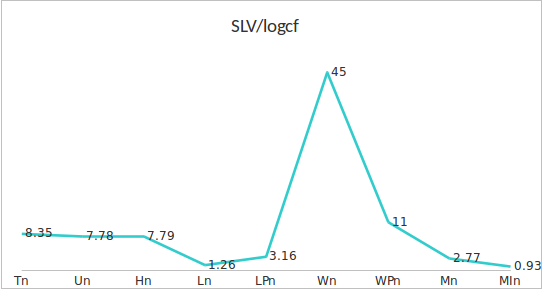
\includegraphics[width=4.4in,height=1.2in]{logcfslv}
		\caption{ Comparison of \froot\ and \SLV\ on benchmarks\label{fig:3}}
	\end{centering}
\end{figure}

\begin{figure}
	\begin{centering}
		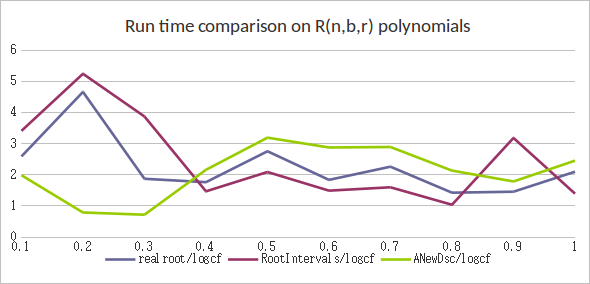
\includegraphics[width=4.4in,height=1.2in]{Rn}
		\caption{ Comparison on random benchmarks $R(n,b,r)$ with different settings\label{fig:2}}
	\end{centering}
\end{figure}

\begin{figure}
	\begin{centering}
		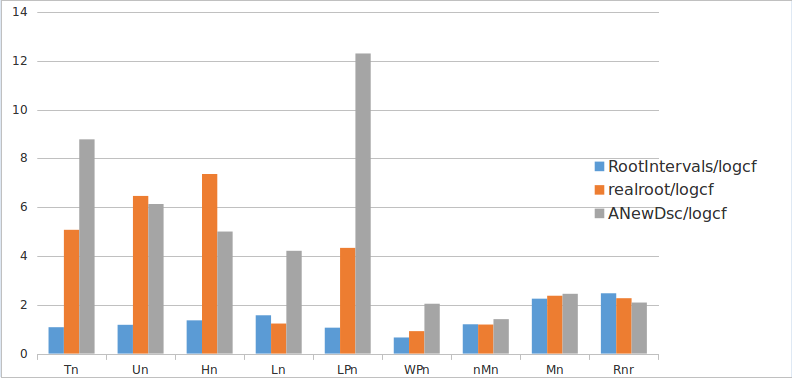
\includegraphics[width=4.4in,height=1.2in]{newresult}
		\caption{ Mean running time compared with \inte, \REALROOT\ and \AND\label{fig:newresult}}
	\end{centering}
\end{figure}

\begin{table}
	\centering
	\captionof{table}{Comparison on three special benchmarks}
	\label{tab:other}
	\begin{tabular}{|| c| c| c| c||}
		\hline
		
		\hline
		\scriptsize{Case}  &\ \  \ \ \ \ \scriptsize{$\frac{\inte }{\froot}$}\ \  \ \ \ \ \  \ \   & \ \ \ \ \  \scriptsize{$\frac{\REALROOT}{\froot}$} \ \ \ \ \  &\ \ \ \  \scriptsize{ $\frac{\AND}{\froot}$ }  \ \ \ \   \\
		\hline
		$W_n$ & 8.7 & 18.04 &  202 \\
		\hline
		$MR_n$ & 0.70 & 980 & 0.174\\
		\hline
		$MI_n$ & 0.58 & 1.89&  0.0029  \\
		\hline
		
		\hline
	\end{tabular}%}
\end{table}

\begin{table}
	\centering
	\captionof{table}{Comparison on $MR_n$}
	\label{tab:and}
	\begin{tabular}{|| c| c| c| c| c ||}
		\hline
		
		\hline
		\scriptsize{Degree}  &\ \  \ \ \ \ \scriptsize{\froot}\ \  \ \  \ \   & \scriptsize{\REALROOT} &\scriptsize{\inte}  &\ \   \ \    \scriptsize{\AND}\ \ \ \   \\
		\hline
		$128$ & 0.016 & 0.734 &  0.015 &  0.02\\
		\hline
		$181$ & 0.018 & 11.154 & 0.031 & 0.038\\
		\hline
		$256$ & 0.034 & 94.849&  0.046  & 0.063\\
		\hline
		$362$ & 0.083 & >600&  0.094 & 0.11\\
		\hline
		$512$ & 0.20 &  >600 & 0.219 & 0.20  \\
		
		\hline
		$724$ & 0.55 &  >600&  0.344 & 0.42 \\
		
		\hline
		$1024$ & 1.46 & >600 & error & 0.79 \\
		
		\hline
		$1448$ & 6.48 &  >600&  error &  1.69 \\
		\hline
		$2096$ & 24.19 &  >600&  error & 3.16 \\	
		\hline
		
		\hline
	\end{tabular}%}
\end{table}

More test results can be found at
	
	 \url{https://github.com/djuanbei/logcf/blob/master/testresult.xls}

In our experiments when {\em Algorithm \ref{alg:up}} is used for computing upper bounds, $T(p)$  takes  more than ninety percent of running time\footnote{The result of  GNU gprof.}.  We have considered methods in \cite{ger04} for computing $T(p)$, but finally we chose the  classical method (Horner's method) for its simplicity. In future work we will use Divide \& Conquer method which is the fastest in \cite{ger04}. We think this will further improve the performance of our tool.

\begin{comment}
\begin{table}
  \centering
  %\tbl{    compare with \cf  \label{tab:open}}{
  \captionof{table}{ compare with \cf\ under old environment } \label{tab:open}
  \begin{tabular}{|| c| c| c|| c|c| c||}
\hline

\hline
\scriptsize{Benchmark}  &\ \  \ \    \ \ \scriptsize{\cf}\ \  \ \  \ \     & \scriptsize{\froot} &\scriptsize{ Benchmark}  &\ \   \ \ \ \  \ \scriptsize{ \cf} \  \  \ \ \ \    \    & \scriptsize{\froot}\\
\hline
$W_{100}$ & 0.054 & 0.01 &  $IW_{100}$ & 0.056 & 0.01\\
\hline
$W_{200}$ & 0.23 & 0.015 & $IW_{200}$ & 0.20 & 0.015\\
\hline
$mW_{100}$ & 0.054 & 0.025& $mIW_{100}$ & 0.14 & 0.01\\
\hline
$mW_{200}$ & 40.5 & 0.16& $mIW_{200}$ & 2.7 & 0.04\\
\hline
$T_{100}$ & 0.52 &  0.01 & $L_{100}$ & 0.80 & 0.02  \\

\hline
$T_{200}$ & 4.32 &  0.13& $L_{200}$ & 7.50 &0.16 \\

\hline
$U_{100}$ & 0.52 &  0.01& $M_{1000}$ & 43.52 & 0.03 \\

\hline
$U_{200}$ & 4.15 &  0.12& $M_{1200}$ & 88 & 0.05 \\

\hline

\hline
  \end{tabular}%}
\end{table}


\begin{figure}
	\begin{centering}
		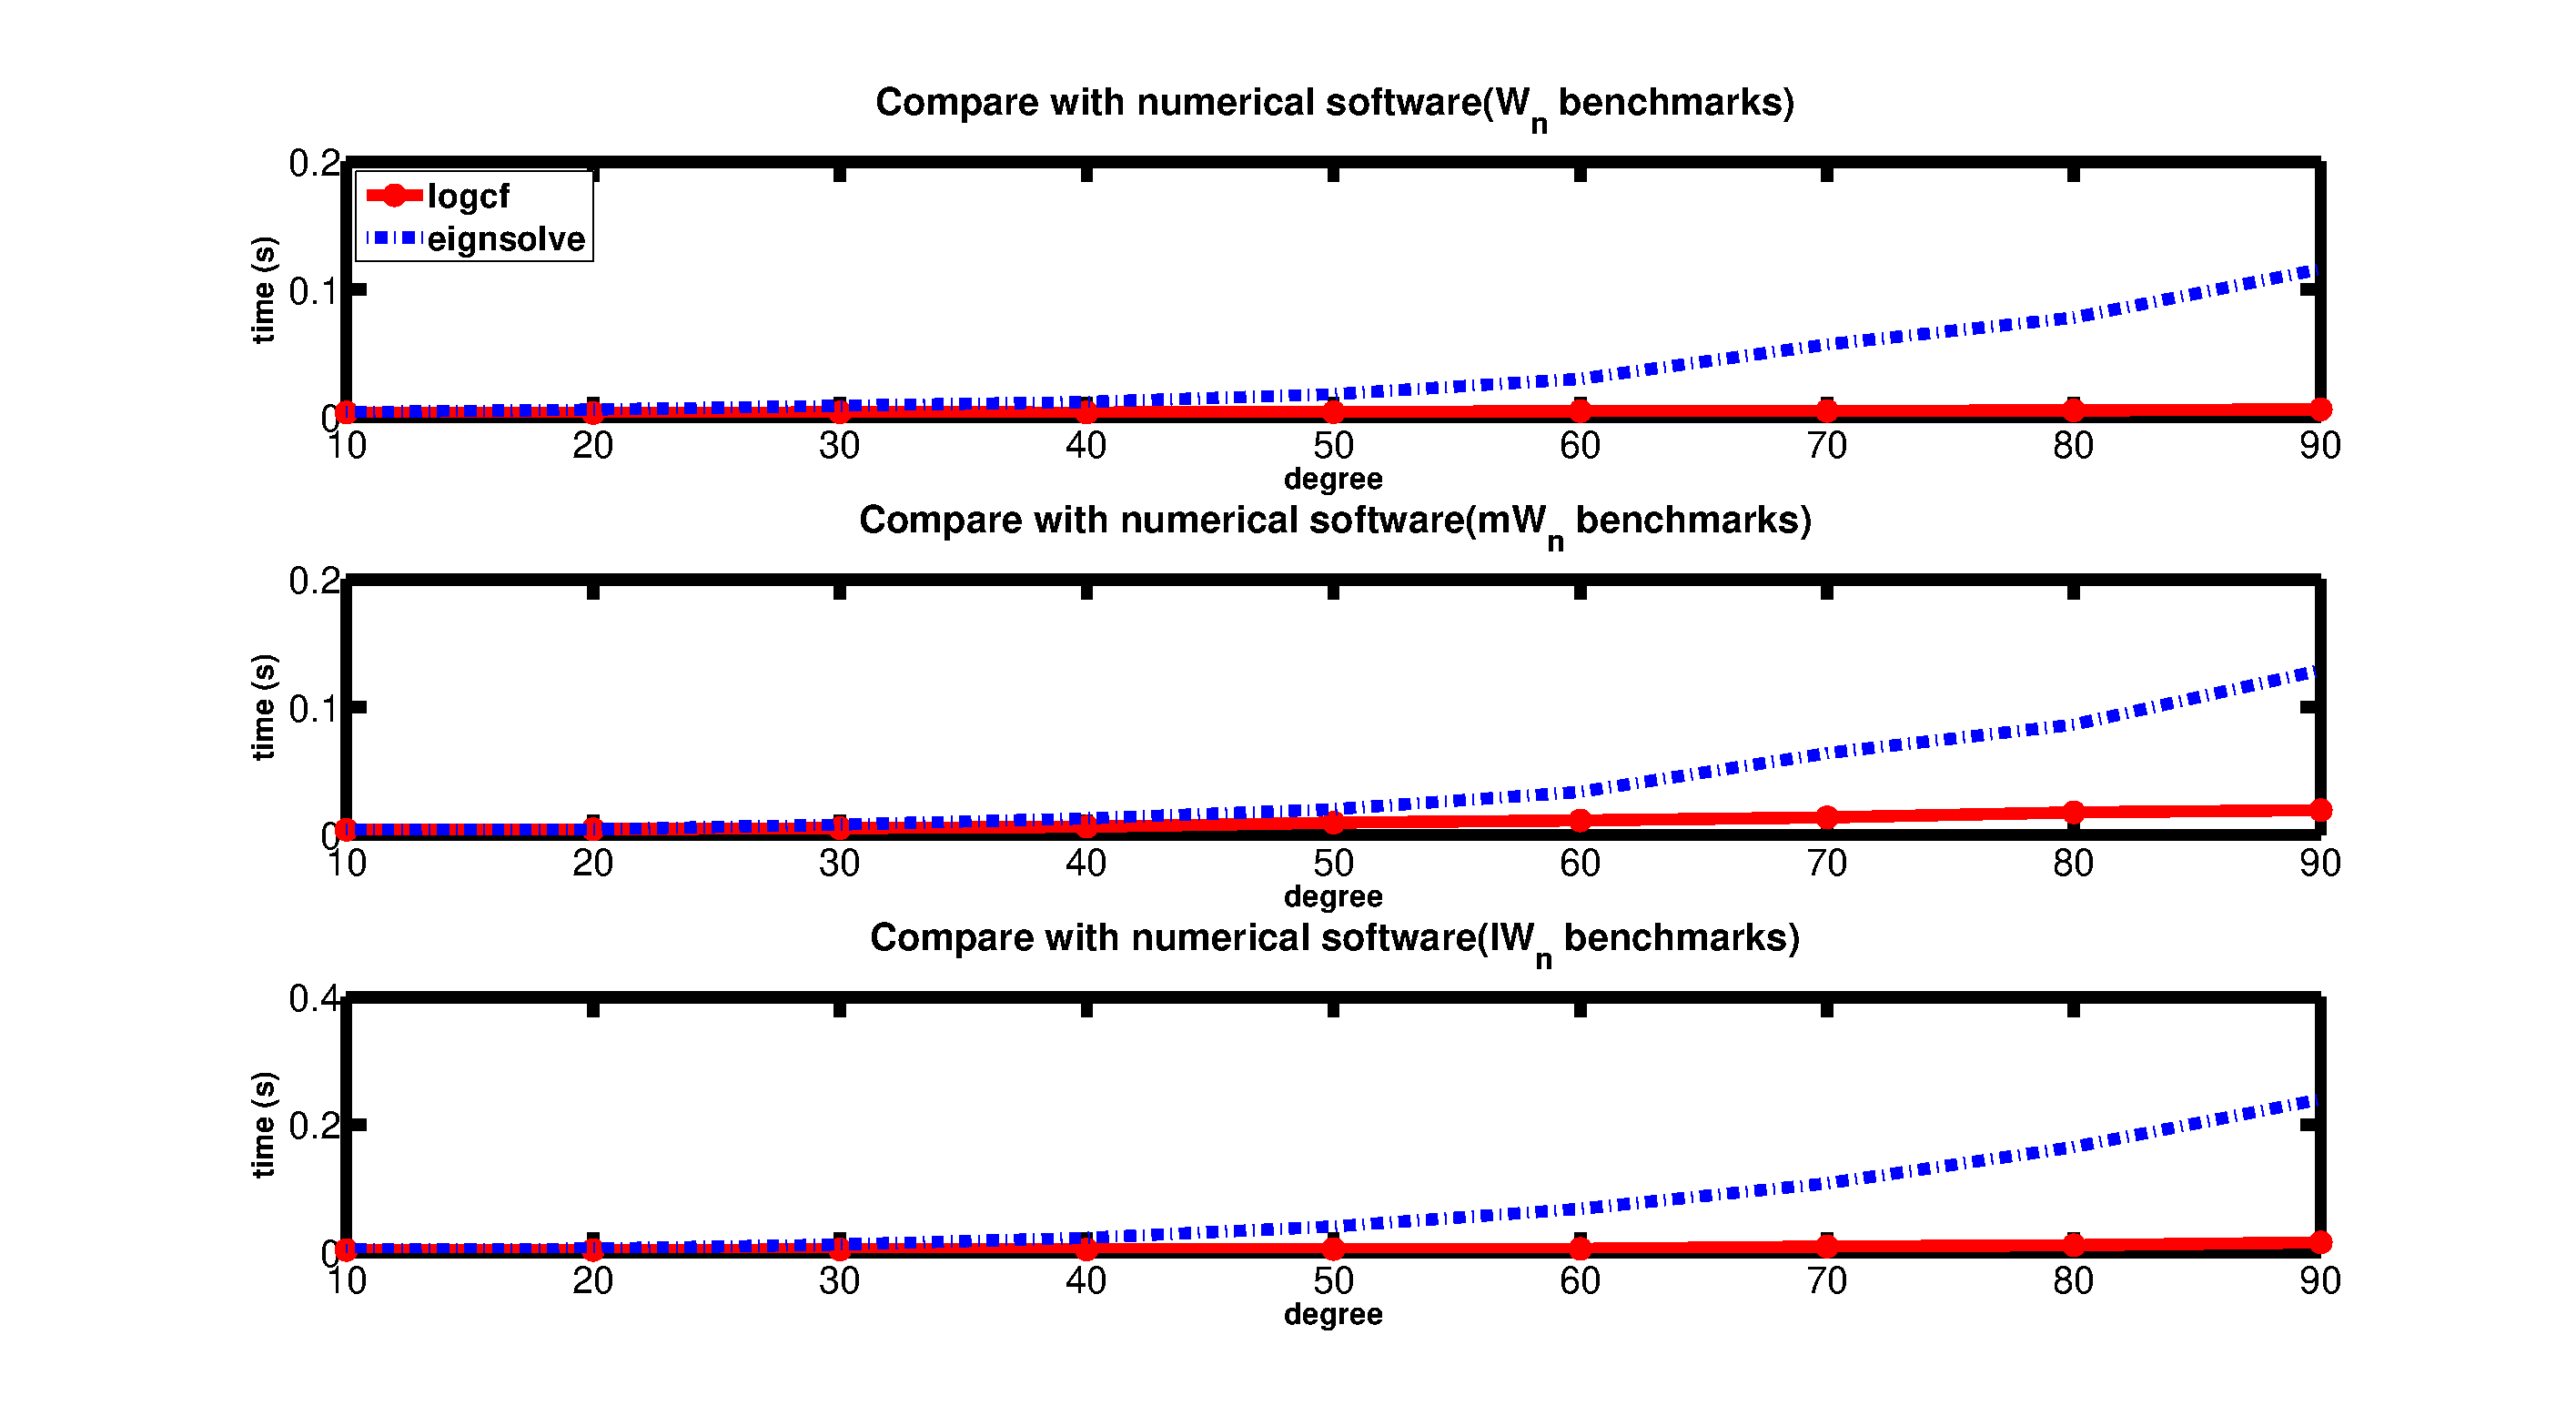
\includegraphics[width=5.4in]{com}
		\caption{ compare with numerical software  \eign\  on old environment\label{fig:1}}
	\end{centering}
\end{figure}

\end{comment}
